\subsection{Backend}
\label{sub:backend}
  In diesem Abschnitt soll beschrieben werden, welche Probleme beim Arbeiten mit dem GTFS Datenformat und einer PostgreSQL Datenbank bestehen und wie diese gelöst sind. Dabei steht vor allem die Behebung von Engpässen bei der Query\footnotemark Performance, als auch die Verringerung der zu verarbeitenden Datenmenge. Sektion \ref{ssub:freiräume_in_der_gestaltung_von_gtfs} beschreibt die generelle Problematik, dass durch die Verwendung des GTFS Formats im Backend entsteht. Die folgenden Abschnitte fokussieren sich darauf dieses Problem zu lösen. Abschnitt "`\nameref{ssub:gtfs_optimierungen}"' zeigt verschiedene GTFS Optimierungsschritte. Darauf folgt die Verbesserung von Polylines in Abschnitt \ref{ssub:polyline_optimieren} und endet mit der Denormalisierung von Datenbanktabellen im letzten Abschnitt \ref{ssub:denormalisierung_der_datenbank}.

  \footnotetext{Ein Query ist eine Informationsanfrage an eine Datenbank} 
  
  % Gliederung eventuell nochmals beschreiben.

  \subsubsection{GTFS Optimierungen}
\label{ssub:gtfs_optimierungen}

  Der erste Schritt um die Performance zu verbessern, ist die Optimierung von GTFS Feeds. Damit lässt sich die Datenmenge bereits vor dem Importieren in die Datenbank, erheblich verringern. Ein Tool um ein GTFS Feed umfassend zu optimieren ist \texttt{gtfstidy} \url{https://github.com/patrickbr/gtfstidy}. Es bietet dabei allerdings nicht nur die Möglichkeit für die Vereinfachung von Polylines sondern kommt mit einer ganzen Reihe an Optimierungsmöglichkeiten. 

  Der Kommandozeilenbefehl \colorbox{materialGrey}{\texttt{\color{white}{\$ gtfstidy -sSiRDeO input.zip output}}} optimiert das Stuttgart-VVS Feed wie folgt:
  
  \begin{itemize}[label={}]
    \item \textbf{-s} Reduziert die Punktanzahl einer Polyline
      
    \item \textbf{-S} Entfernt redundante Polylines.

    \item \textbf{-i} Umwandlung von Zeichen ID's (String) in Zahlen ID's (Integer).\footnote{Aus der String ID \texttt{'1.T0.10-1-j17-1.16.H'} wird \texttt{78}}

    \item \textbf{-O} Entfernt Feed Einträge die nicht referenziert werden.

    \item \textbf{-R} Entfernt doppelt vorhandene Routen.

    \item \textbf{-e} Setzt fehlerhafte oder optionale Felder auf einen Standard Wert.

    \item \textbf{-D} Entfernt fehlerhafte Einträge aus dem Feed.
  \end{itemize}

  Durch Verwendung von gtfstidy konnte das Feed optimiert werden und die Datengröße der einzelnen Dateien um folgendes Maß verringert werden.

  \begin{longtable}{|>{\raggedright \arraybackslash}p{5.0cm}|>{\raggedright \arraybackslash}p{5.0cm}|>{\raggedright \arraybackslash}p{5.0cm}|}
    \hline
    Dateiname & Größe davor& Größe danach\\
    \hline
    trips.txt & 6 MB & 2.8 MB\\
    stop\_times.txt & 103 MB & 53 MB\\
    stops.txt & 651 KB & 355 KB\\
    shapes.txt & 77.3 MB & 22.4 MB\\
    routes.txt & 54 KB & 38 KB\\
    calendar\_dates.txt & 557 KB & 463 KB\\
    \hline
    \caption{Tabellengröße bevor und nach anwenden von gtfstidy}
    \label{tbl:gtfs_tidy_results}
  \end{longtable}

  Insgesamt konnte so die Größe des Feeds von 79 MB auf 118 MB um knapp 50\% verringert werden. Vor allem die Umwandlung von langen String ID's in kürzere Integer ID's trägt maßgeblich zur Verringerung der Dateigröße bei.

% subsubsection gtfs_optimierungen (end)
  \subsubsection{Polyline optimieren}
\label{ssub:polyline_optimieren}

  Die Optimierung der Polyline ist ein sehr wichtiger Aspekt in meiner Arbeit und soll in diesem Abschnitt vertieft werden.

  \subsubsection*{Ramer–Douglas–Peucker}
  \label{ssub:ramer_douglas_peucker}
    Das Problem: Die im Stuttgart-VVS Feed zur Verfügung gestellten Polylines sind Überdefiniert und können aus tausenden Punkten bestehen. Für eine Visualisierung ist eine solche Genauigkeit nicht notwendig und aufgrund der großen Datenmenge problematisch. Im vorigen Abschnitt \ref{ssub:gtfs_optimierungen} wurde die Option \colorbox{materialGrey}{\texttt{\color{white}{-s}}} vorgestellt. Dieser Befehl verwendet den "`Ramer–Douglas–Peucker"' (RDP) Algorithmus um die Anzahl der Punkte einer Polyline zu reduzieren. Der Vorteil besteht darin, dass dabei nicht der Linienverlauf verändert wird. Abbildung~\ref{fig:simplify} zeigt ein Beispiel einer solchen Vereinfachung mittels einer JavaScript Bibliothek\footnote{Simplify.js \url{http://mourner.github.io/simplify-js/}}.

    \begin{figure}[htbp]
      \centering
      \subfloat[Polyline vor RDP]{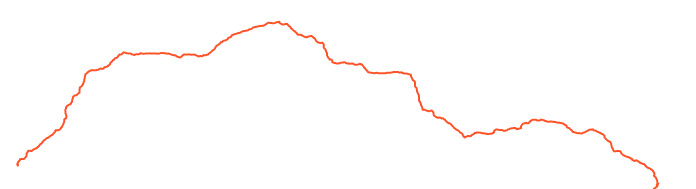
\includegraphics[width=0.48\textwidth]{simplify_before.jpg}\label{fig:simplify_before}}
      \hfill
      \subfloat[Polyline nach RDP]{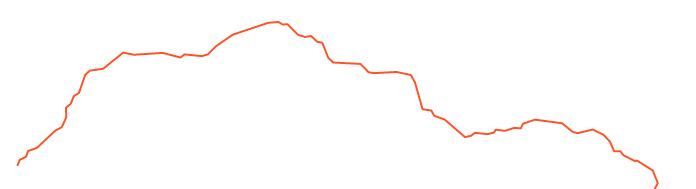
\includegraphics[width=0.48\textwidth]{simplify_after.jpg}\label{fig:simplify_after}}
      \caption{Vereinfachung einer Polyline mittels Simplify.js}
      \label{fig:simplify}
    \end{figure}

    Ausgangspunkt ist eine Polyline mit $\approx1000$ Punkten (\ref{fig:simplify}a). Nach der Vereinfachung (\ref{fig:simplify}b) ist die Anzahl auf 100 Punkte reduziert, ohne dabei visuell merklich einzubüßen. Dies ist eine erhebliche Reduzierung der Punkte um 90\%. Wie wirkt sich dieser Algorithmus positiv auf das Projekt aus? Die Vorteile sind weitreichend. Sehen wir uns die Shape Tabelle in Abbildung \ref{fig:shape_simplify} an. \ref{fig:shape_simplify}a zeigt 394 Reihen vor der Optimierung und nur noch 140 (\ref{fig:shape_simplify}b) nach Anwendung von gtfstidy.

    \begin{figure}[htbp]
      \centering
      \subfloat[Shapte Tabelle vor RDP]{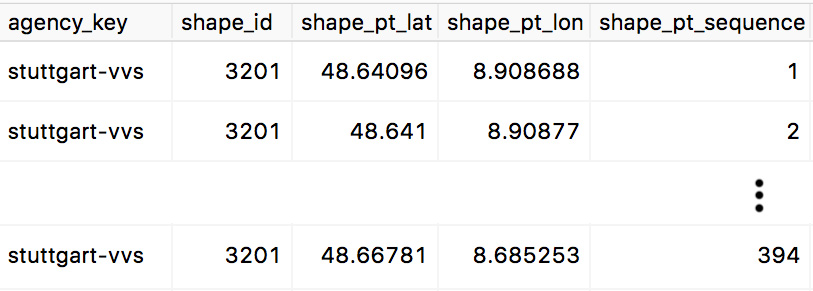
\includegraphics[width=0.48\textwidth]{shape_simplify_before.jpg}\label{fig:shape_simplify_before}}
      \hfill
      \subfloat[Shapte Tabelle nach RDP]{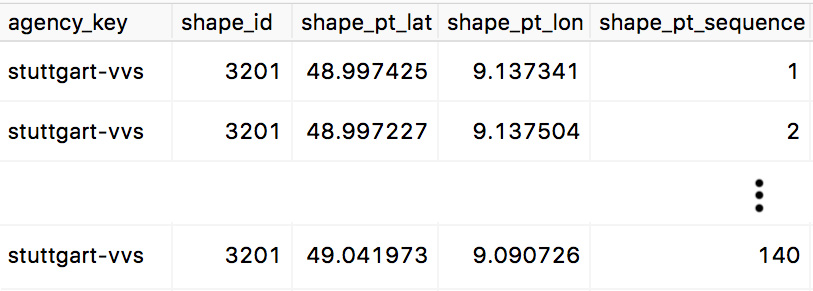
\includegraphics[width=0.48\textwidth]{shape_simplify_after.jpg}\label{fig:shape_simplify_after}}
      \caption{Reduzieren der Polyline via gtfstidy}
      \label{fig:shape_simplify}
    \end{figure}

    In seinem Originalzustand hat das verwendete VVS Feed 1,085,859 Mio Zeilen. Nach der Anwendung sind diese auf 617,653 Tsd. verringert. Testet man folgende PostgreSQL Abfrage
    \colorbox{materialGrey}{\texttt{\color{white}{{\color{materialBlue}SELECT} * {\color{materialBlue}FROM} gtfs\_shapes {\color{materialBlue}WHERE} shape\_id = {\color{materialRed}3201}}}}
    die alle Punkte einer Polyline ausgeben soll, so ergibt sich für ein optimiertes Feed eine Query Zeit von $\approx145 ms$ und für das nicht optimierte Feed $\approx250 ms$. Schon durch diese einfache Methode sind bereits erste Performance Steigerungen wahrnehmbar.

  % subsubsection ramer_douglas_peucker (end)

  \subsubsection*{Aggregieren der Shape Tabelle}
  \label{ssub:aggregieren_der_shape_tabelle}
    In GTFS wird für jeden Punkt einer Polyline eine Reihe in der Datenbank belegt. Diese Abfolge ist durch eine sogenannte \texttt{Shape Point Sequence} festgelegt, was nichts anderes ist als eine Zahl von $1$ bis $n$. Dies ist auch bereits in obiger Tabelle \ref{fig:shape_simplify} zu sehen gewesen. Sehr viel effektiver wäre es allerdings, diese Punkte nicht Reihenweise zu speichern, sondern alle zusammen gehörenden Punkte in einem einzigen Feld zu speichern. Dies ist in PostgreSQL durch eine Aggregierung möglich. Daraus ergibt sich folgende Shape Tabelle:

    \begin{figure}[htbp]
      \begin{center}
        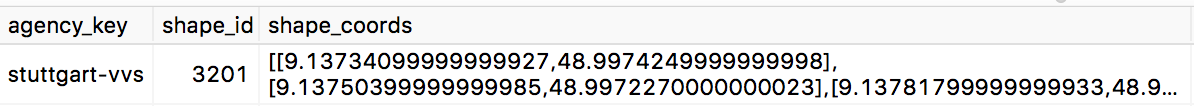
\includegraphics[width=\textwidth]{aggregated.png}
        \caption{Aggregierte Koordinaten der Shape Tabelle}
        \label{fig:aggregated}
      \end{center}
    \end{figure}

    Wie zu sehen ist benötigt nun eine Polyline in der Shape Tabelle nicht mehr 140 Reihen, sondern nur noch eine einzige. Für diese Arbeit ist dies auf alle Polylines angewendet worden und in einer neuen Tabelle namens \texttt{denormalized\_shapes} abgespeichert. Dadurch ist die Berechnung der Aggregierung nur einmal nötig. Der SQL-Befehl dafür ist dem Anhang unter \ref{lst:sql_aggregate_shape}. zu entnehmen.
    Wenden wir die selbe SQL Abfrage, die bereits oben Verwendung fand, auf die neue \texttt{denormalized\_shapes} Tabelle an. Die Query Zeit ist auf $\approx1ms$ gesunken! Anstatt hunderte Reihen muss nur eine einzige Reihe ausgelesen werden, was sehr sehr schnell ist. Durch das Denormalisieren\footnotemark der Shape Tabelle ist auch die Anzahl der Reihen auf ein Minimum gesunken. Von den früheren 617,653 Tsd. Reihen, sind jetzt durch die Aggregation nur noch 4,524 Tsd. übrig.

    \footnotetext{Denormalisieren beschreibt den Prozess der Relationsauflösung von Datenbanktabellen.}
  
  % subsubsection aggregieren_der_shape_tabelle (end)

  \subsubsection*{Polyline Encoding}
  \label{ssub:polyline_encoding}
    Die letzte Maßnahme zur Optimierung der Polyline stellt das sogenannte Polyline Encoding dar. Wie dieses Verfahren genau funktioniert, geht an dieser Stelle zu weit. Hier soll nur erklärt werden, was das Polyline Encoding für diese Arbeit bedeutet und warum es verwendet wird.\\

    Das Polyline Encoding kann in JavaScript beispielsweise durch das Google-Polyline\footnote{\url{https://www.npmjs.com/package/google-polyline}} Paket eingesetzt werden. Das Encoding wandelt eine Polyline, bestehend aus Punkten, in einen String um. Zum Beispiel die Punkte: (38.5, -120.2), (40.7, -120.95), (43.252, -126.453) werden als
    \colorbox{materialGrey}{\texttt{\color{white}{\_p\textasciitilde iF\textasciitilde ps|U\_ulLnnqC\_mqNvxq`@}}}
    codiert. Dies geschieht in meiner Anwendung immer genau dann, bevor Daten von Server in Richtung Client geschickt werden: Encode $\rightarrow$ Send $\rightarrow$ Decode. Da eine codierte Polyline weniger Zeichen benötigt, kann damit Datenvolumen bei der Kommunikation zwischen Server und Client gespart werden.

  % subsubsection polyline_encoding (end)


% subsubsection polyline_optimieren (end)
  \subsubsection{Denormalisierung der Datenbank}
\label{ssub:denormalisierung_der_datenbank}
  Die Denormalisierung ist eine Strategie, die auf eine zuvor normalisierte Datenbank angewendet wird, um die Leistung zu erhöhen. Die Denormalisierung ist der Prozess, bei dem versucht wird, die Leseperformance einer Datenbank zu verbessern, auf Kosten der Schreibleistung, durch Hinzufügen redundanter Kopien von Daten oder durch deren Gruppierung.\parencite{sanders}
  Der große Nachteil von Denormalisierung, nämlich die Redundanz von Daten, spielt für dieses Projekt keine Rolle, da die Daten ausschließlich ausgelesen und nicht geschrieben werden. Was bleibt sind die Vorteile.\\

  Für dieses Projekt bedeutet diese Methode, eine neue Tabelle zu generieren, die den Zugriff auf die benötigten Daten einfach macht. Im Grunde handelt es sich um eine Vorberechnung. Anstatt die Tabellen bei jeder Anfrage an den Server aufwendig über viele \texttt{SQL-JOINS} zu verknüpfen, wird diese Verknüpfungen einmalig vorberechnet und in eine Tabelle gespeichert. Eine Denormalisierung  einer Tabelle ist bereits im vorherigen Abschnitt "`\nameref{ssub:aggregieren_der_shape_tabelle}"' gezeigt und führte dazu, dass die Polyline über die Abfrage einer einzigen Tabellenreihe erhalten werden kann was die Performance signifikant erhöhte. Zur besseren Verständnis soll folgende Grafik helfen:

  \begin{figure}[htbp]
    \begin{center}
      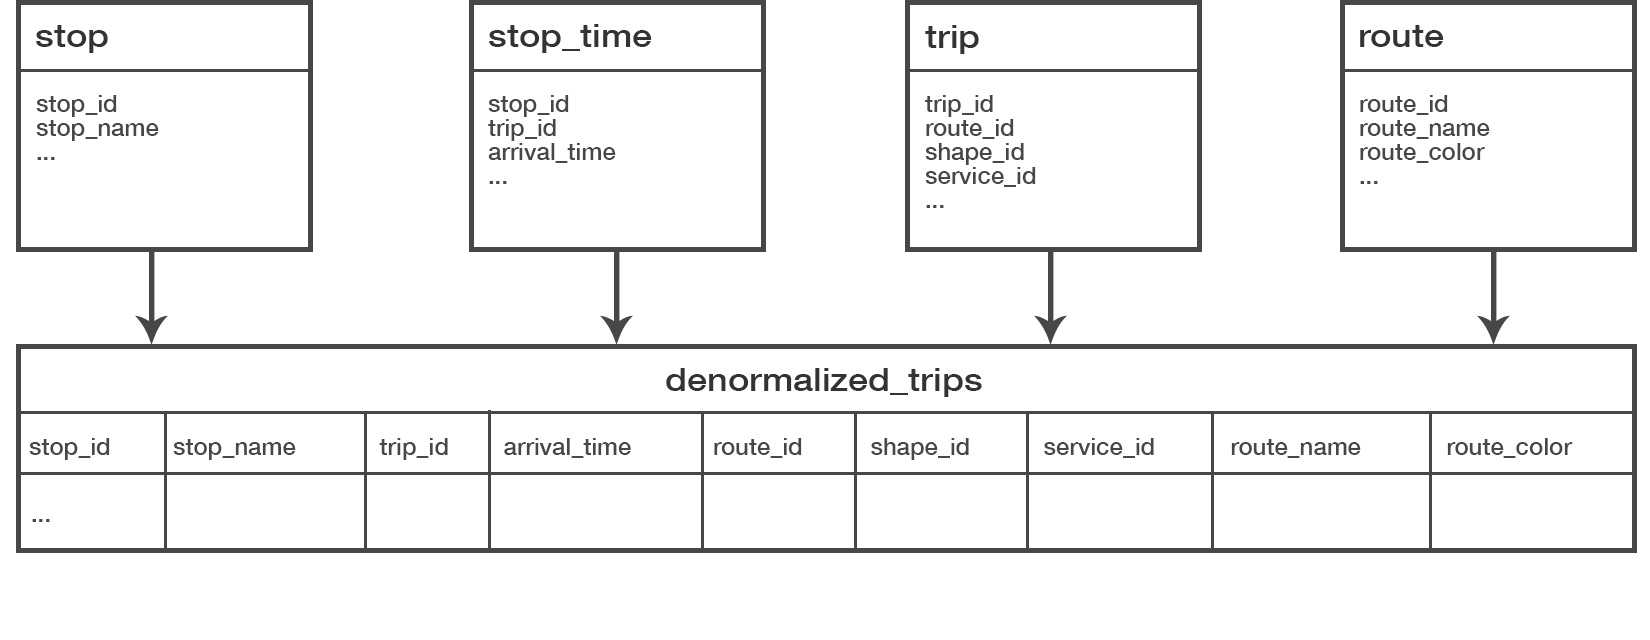
\includegraphics[width=\textwidth]{denormalizing.jpg}
      \caption{Beispiel einer Denormalisierung von Tabellen}
      \label{fig:denormalizing}
    \end{center}
  \end{figure}

  Wie in Abbildung \ref{fig:denormalizing} zu sehen ist, wird aus einer vertikalen Anordnung der einzelnen Datenfelder, eine horizontale Anordnung in einer einzigen \texttt{denormalized\_trips} Tabelle. Eine Reihe in dieser neuen Tabelle steht für genau einen Eintrag eines Trips. Anstatt also bei jeder Anfrage an den Server die verschiedenen Daten mittels \texttt{JOIN} verknüpfen zu müssen, können diese jetzt per Zugriff auf eine einzige Reihe in nur einer Tabelle erfragt werden.\\

  Dieses Prinzip, der Gruppierung von Daten in einer neuen Tabelle soll nun auch auf die anderen benötigten Tabellen angewendet werden. Die Denormalisierung erfolgt in 3 Schritten:

  \begin{enumerate}
    \item Erstellen der neuen Tabelle \texttt{denormalized\_trips}
    \item Importieren der verschiedenen Daten in diese neue Tabelle
    \item Mögliche Abfragen sind nun über diese neue Tabelle möglich.
  \end{enumerate}

  Das SQL-Statement ist abermals aufgrund seiner Länge Anhang \ref{lst:denormalized_shapes} zu entnehmen. Dies resultiert in einer Tabelle die wie folgt aussieht:

  \begin{figure}[htbp]
    \begin{center}
      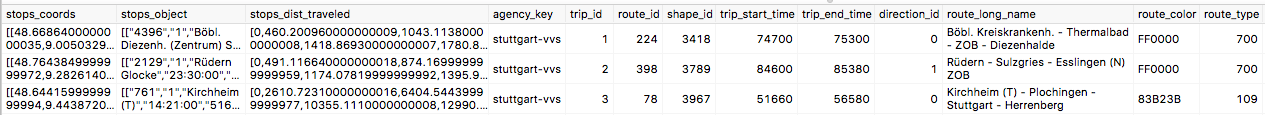
\includegraphics[width=\textwidth]{denormalized_tables.png}
      \caption{Auszug aus der \texttt{denormalized\_trips} Tabelle}
      \label{fig:denormalized_table}
    \end{center}
  \end{figure}  

  \subsubsection*{Ergebnisse der Denormalisierung}
  \label{ssub:ergebnisse_der_denormalisierung}
    Für die Visualisierung ist eine Abfrage der aktiven Trips am wichtigsten.
    Folgende Tabellen werden für die Abfrage benötigt.

    \begin{figure}[htbp]
      \begin{center}
        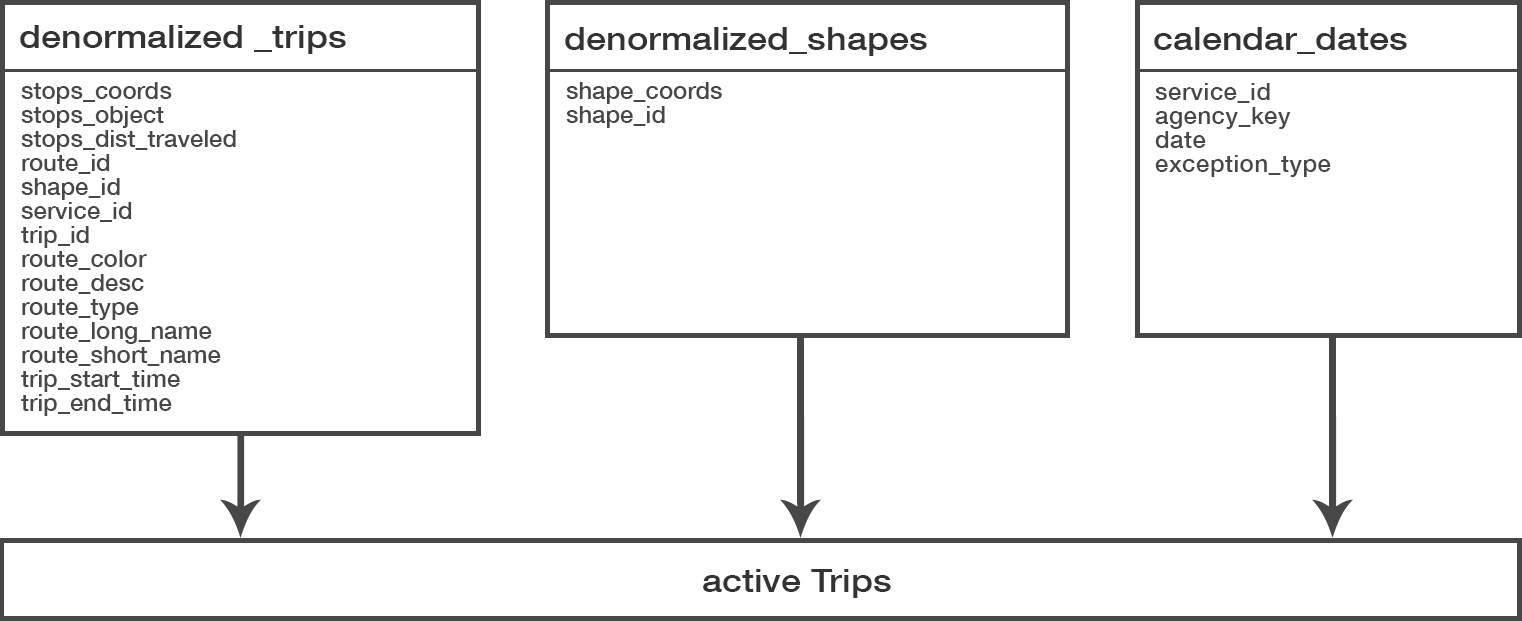
\includegraphics[width=\textwidth]{denormalizing_results.jpg}
        \caption{Benötigte Tabellen zur Abfrage von Trips}
        \label{fig:denormalizing_results}
      \end{center}
    \end{figure}

    Wie zu sehen ist, wird auf die Denormalisierte \texttt{Shape} und \texttt{Trips} Tabelle zugegriffen.

    Nachfolgend die Ergebnisse für die Abfrage von Trips in einem wachsenden Zeitrahmen. Die verwendete SQL-Abfrage befindet sich im \nameref{sec:anhang} unter Listing \ref{lst:query_trips}.

    \begin{longtable}{|>{\raggedright \arraybackslash}p{5.0cm}|>{\raggedright \arraybackslash}p{5.0cm}|>{\raggedright \arraybackslash}p{4.0cm}|}
    \caption{Evaluierung der Denormalisierung}\label{tbl:evaluierung_der_denormalisierung}\\
      \hline
        Zeitraum & Trip Anzahl & Query Zeit\\
      \hline
        9:00 bis 9:15 & 88 & 98 ms\\
        9:00 bis 10:00 & 1125 & 154 ms\\
        9:00 bis 12:00 & 3360 & 285 ms\\
        9:00 bis 15:00 & 7070 & 497 ms\\
        9:00 bis 21:00 & 14718 & 900 ms\\
      \hline
    \end{longtable}

    Die Ergebnisse Zeigen, dass die Abfragezeit der Datenbank für die aktiven Trips erheblich gesunken ist. Anfangs ist solch eine Anfrage aufgrund der endlosen Laufzeit erst gar nicht möglich gewesen.

    \begin{figure}[htbp]
      \begin{center}
        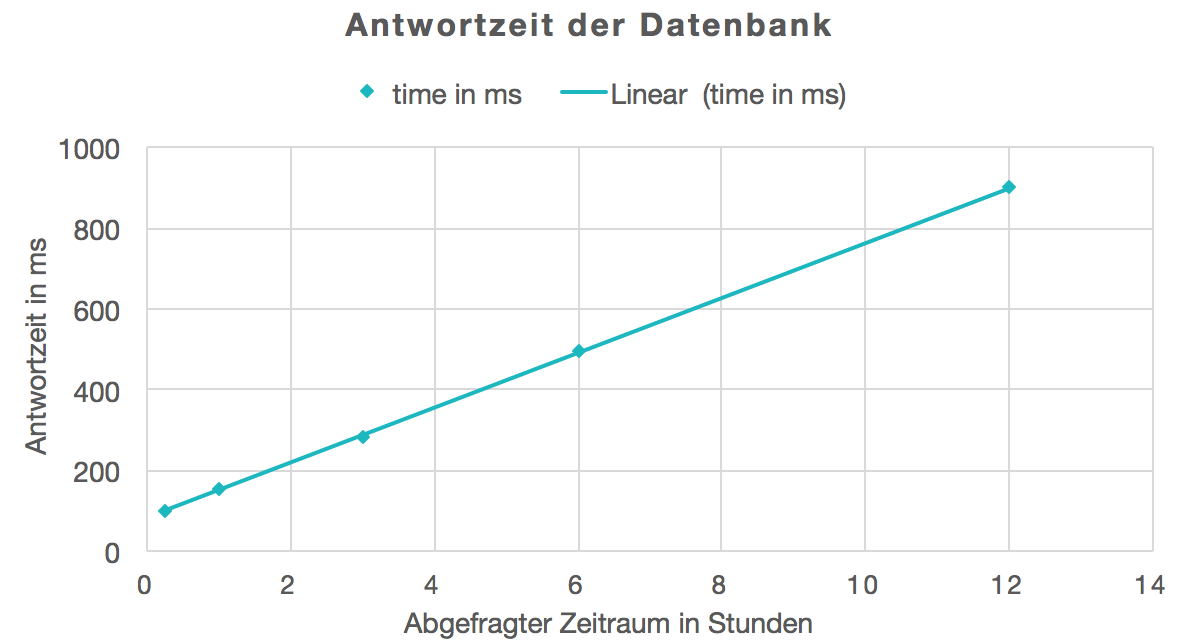
\includegraphics[width=0.65\textwidth]{query_time_chart}
        \caption{Plot der Abfragezeiten}
        \label{fig:query_time_chart}
      \end{center}
    \end{figure}
    
    Abbildung \ref{fig:query_time_chart} zeigt einen Plot der Query Zeit aus Tabelle \ref{tbl:evaluierung_der_denormalisierung} als nahezu linearen Graphen. Daraus folgt, dass die Antwortzeit der Datenbank linear mit dem abgefragten Zeitraum wächst. In der Visualisierung sind vor allem Trip Abfragen zwischen einer Minute und einer Stunde in Verwendung. Die Abfragezeit bewegt sich damit zwischen $\approx 80 -  160\; ms$.
    
  % subsubsection ssub:ergebnisse_der_denormalisierung (end)

% subsubsection denormalisierung_der_datenbank (end)
  \subsubsection{API Endpunkte}
\label{ssub:api_endpunkte}
  Um einen Datenaustausch zwischen Server und Client zu ermöglichen, sind folgende API\footnotemark Endpunkte vorhanden. 

  \footnotetext{Application Programming Interface}

  \begin{itemize}[label={}]
    \item \textbf{/daily} Stellt die Daten für das Zeitstrahldiagramm bereit. Wird beim Start der Anwendung einmalig Angefragt. Die Antwort enthält XY-Wertpaare. X stellt dabei die Zeit in Sekunden und Y die zu diesem Zeitwert aktiv werdenden Trips dar.

\begin{lstlisting}[captionpos=t, caption=Antwort des Servers zur Anfrage \texttt{/daily}, label=lst:daily_response]
[
  {"x":86340,"y":"6"},
  {"x":86400,"y":"10"}, 
  ...
]
\end{lstlisting}

    \item \textbf{/trips/:from,:to} Ermöglicht das Abfragen von Trips, die in einer Zeitspanne \texttt{from - to} aktiv sind. Beim initialen Aufruf der Webanwendung wird dieser Endpunkt als erstes angefragt um die aktiven Trips innerhalb einer Stunde zu bekommen. Der gewählte Zeitraum ist in Sekunden anzugeben. Die Definition ist wie folgt: $t_{from} = now$ und $t_{to} = now + 600 sec$. Die Sekunden lassen sich nach der Formel aus Kapitel \ref{ssub:time} berechnen.
     durch das Addieren der Stunden, Minuten und Sekunden errechnen. Bsp: 17:04:59 Uhr

    $\Rightarrow t_{from} = 61499 \Rightarrow t_{to} = 61499 + 600\;sec$ $\Rightarrow$ \texttt{/trips/61499,62099}

    Die Antwort des Servers auf einen Endpunkt vom Typ \texttt{/trips/} ist ein Objekt mit der Trip\_Id, dessen Inhalt der \texttt{GeoJSON} spezifikation nach RFC 7946 folgt:

\begin{lstlisting}[captionpos=t, caption=Trip Objekt, label=lst:trip_object]
{
  2498: {  
    "type": "FeatureCollection",
    "features": [
      {
        "type": "Feature",
        "properties": {
          "name": "shape",
          ...
        },
        "geometry": {
          "type": "LineString",
          "coordinates": [[9.4437,48.64482], ...]
        }
      },
      {
        "type": "Feature",
        "properties": {
          "name": "station"
        },
        "geometry": {
          "type": "Point",
          "coordinates": [9.443688, 48.6448]
        }
      },
      ...
    ]
  }
}
\end{lstlisting}
  
    Da die Antwort in Listing \ref{lst:trip_object} mittels "`..."' gekürzt ist, sind detailiertere Antworten im \nameref{sec:anhang} unter Listing \ref{lst:geojson_featurecollection}, \ref{lst:shape_feature} und \ref{lst:station_feature} zu finden.
  

    \item \textbf{/trips/:id} Antwortet mit den zur ID gehörenden Trip Informationen. Dieser Endpunkt ermöglicht es, Informationen für nur einen einzigen Trip zu bekommen. Dies ist vor allem dann hilfreich, wenn der Nutzer ein Vehilce anklickt und Informationen über diesen Trip angezeigt bekommen möchte. Beispiel: \texttt{/trips/51295}

    \item \textbf{/trips/new/:from,:to,:tripIds} Stellt die Abfrage für neue Trips zur Verfügung und exkludiert dabei diejenigen Trips, die in \texttt{:tripIds} genannt sind. Damit wird verhindert, dass bereits auf der Karte vorhandene Trips nicht doppelt auftauchen können. Dieser Query wird in einem 30 Sekunden Intervall vom Client an den Server gesendet um die neusten Trips zu erhalten. Damit wird die Karte aktuell gehalten. Beispiel: Es ist 10:00 Uhr, hole die in der nächsten Minute aktiv werdenden Trips (Zeitraum 10:00 bis 10:01 Uhr) und schließe die Trips mit der ID \texttt{51295,9212,52} vom Ergebnis aus \texttt{/trips/new/36000,36060,51295,9212,52}.

    \item \textbf{/trips/new/:from,:to} Stellt die gleiche Funktionalität wie der vorherige Endpunkt zur Verfügung, mit der Ausnahme, dass keine Trip-ID's übermittelt werden müssen. Dieser Endpunkt ist beispielsweise dafür da, falls die Karte leer ist und noch keine aktiven Trips enthält.

  \end{itemize}

% subsubsection api_endpunkte (end)
  \subsubsection{Server}
\label{ssub:server}
  Der Nodejs Server stellt die zuvor definierten Endpunkte mittels \texttt{Express.js} als ansprechbare Routen dem Client zur Verfügung. Express ist ein minimalistisches Node.js Framework für moderne Web Applikationen. Es vereinfacht die Erstellung von API Endpunkten durch das Bereitstellen hilfreicher Methoden zur Erstellung von Routen\footnotemark.

  \footnotetext{Routing refers to determining how an application responds to a client request to a particular endpoint, which is a URI (or path) and a specific HTTP request method (GET, POST, and so on). \url{https://expressjs.com/en/starter/basic-routing.html}}

  \begin{figure}[htbp]
    \begin{center}
      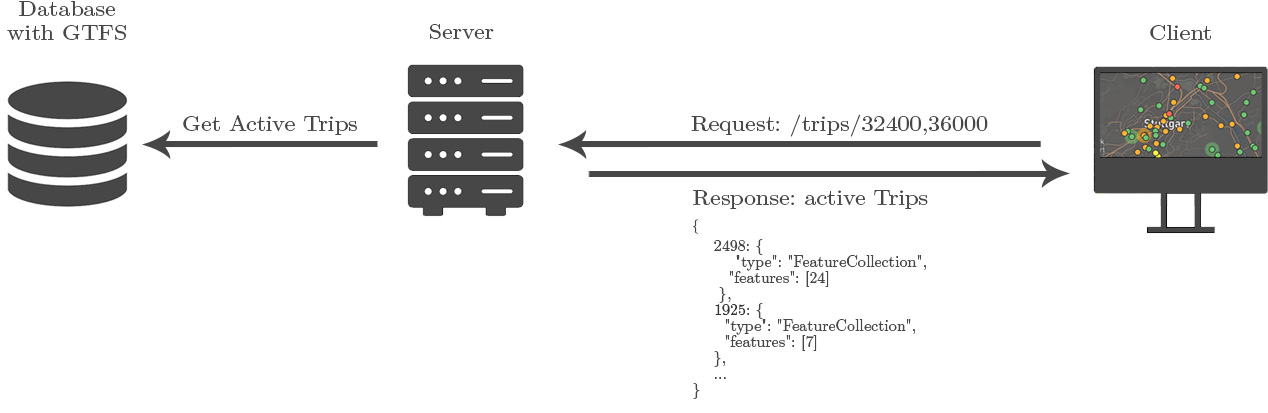
\includegraphics[width=\textwidth]{server_client.jpg}
      \caption{Server / Client Relation}
      \label{fig:server_client}
    \end{center}
  \end{figure}

  Trifft eine valide Anfrage auf den \texttt{/trips/:from,:to} Endpunkt, so wird ein Ablauf nach Abbildung \ref{fig:server_client} angestoßen.
  Die eintreffenden Anfragen werden vom Server entgegengenommen, validiert, verarbeitet und anschließend die entsprechende Antwort zurück gesendet. Die Validierung prüft die vom Client übergebenen Parameter auf ihre Plausibilität. Schlägt diese Prüfung fehl wird ein Fehler vom Server zurückgegeben und der Server wartet auf eine neue Anfrage. Die wichtigste Routine des Servers stellt die Abfrage von Trips aus der Datenbank dar. Die Datenbank sucht diejenigen Trips heraus, welche in dem benötigten Zeitraum \texttt{from, to} aktiv sind. Dabei wird das Datum und der Wochentag zum Zeitpunkt der Anfrage verwendet. Damit der Client bei der Animation möglichst wenig Rechenarbeit hat, werden alle Daten, bei denen dies möglichst ist, vorberechnet. Folgender Ablauf findet statt:

  \begin{itemize}
    \item \textbf{Daten Mapping:} Die Trips aus der Datenbank werden in das \texttt{GeoJSON}-Format umgewandelt, damit diese im weiteren Programmverlauf einfacher zu verarbeiten sind. Dabei werden die im Kapitel "`\ref{sub:begriffe} \nameref{sub:begriffe}"' festgelegten Definitionen beachtet.

    \item \textbf{Zurückgelegte Distanz:} Damit eine Animation der Vehicle stattfinden kann ist die Berechnung der Distanzen zwischen den einzelnen Stationen nötig. Falls das Feld \texttt{stops\_dist\_traveled}\footnotemark in der Datenbank vorhanden ist, kann die zurückgelegte Distanz sehr einfach daraus berechnet werden. Ist dies nicht der Fall so wird ein Station Matching durchgeführt, um die Distanzen berechnen zu können.
    \footnotetext{Die zurückgelegte Distanz bis zu einer Station $S$}

    \item \textbf{Station Matching:} Unter Station Matching versteht sich die Positionierung der Stationen auf und entlang der Polyline. Dies wird im nächsten Abschnitt ausführlicher betrachtet.

    \item \textbf{Feststellen der Richtung:} Für eine Polyline ist es unerheblich ob die Koordinaten in der Reihenfolge $\{ p_1, p_2, \dotsc, p_n \}$ oder $\{ p_n, \dotsc, p_2, p_1 \}$ angeordnet sind. Damit das Vehicle aber in die richtige Richtung von $A$ nach $B$ fährt, ist es wichtig dass die Koordinaten der Polyline in aufsteigender Reihenfolge festgelegt werden. Falls dies nicht er Fall ist, werden die Koordinaten in ihrer Reihenfolge umgekehrt.

    \item \textbf{Codieren der Polyline:} Zuletzt werden die Koordinaten in einen Polyline String Codiert und abschließend versendet.
  \end{itemize}

% subsubsection server (end)
  \subsubsection*{Station Matching}
\label{ssub:station_matching}

  Das Station Matching war eines der fundamentalen Herausforderungen bei der Programmierung des Servers. Es ist dafür da, um die Distanz zwischen den einzelnen Stationen zu ermitteln. Zwar hat das Stuttgart-VVS Feed ein \texttt{stop\_distance\_traveled} Feld, welches die benötigten Distanz Informationen direkt aus der Datenbank liefert, aber für andere GTFS-Feeds die getestet wurden, ist dieses Feld oftmals nicht vorhanden. Die Applikation verwendet also das \texttt{stop\_distance\_traveled} Feld, falls es vorhanden ist und als Fallback-Lösung erfolgt die Berechnung via Station Matching Algorithmus.\\

  Das Station Matching soll folgendes Problem lösen:

  \begin{figure}[htbp]
    \begin{center}
      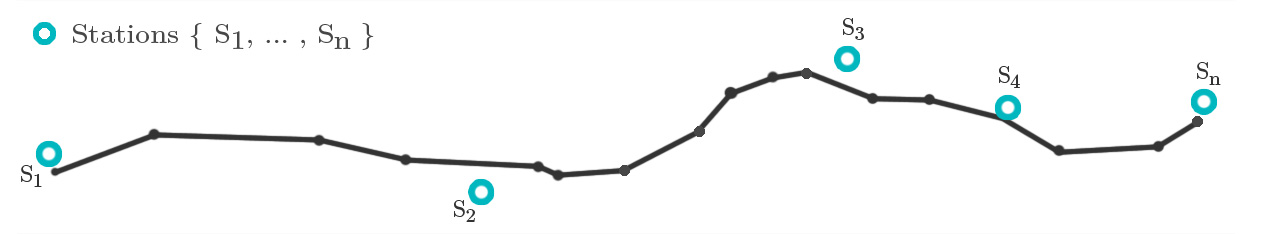
\includegraphics[width=\textwidth]{station_problem.jpg}
      \caption{Stationen liegen nicht direkt auf der Polyline}
      \label{fig:station_problem}
    \end{center}
  \end{figure}
  
  Wie in Grafik \ref{fig:station_problem} zu sehen ist liegen die Stationen nicht exakt auf der Polyline, sondern sind ein wenig abseits platziert. So entspricht die Position der Station einer Haltestelle oder Bahnhof. Meistens befinden sich diese ein wenig versetzt zum eigentlichen Verlauf der Strecke. Die Visualisierung interpoliert die Bewegung eines Vehicles zwischen den einzelnen Stationen. Damit das möglich ist, wird die zurückzulegende Distanz zwischen den einzelnen Stationen benötigt. Um sie zu berechnen ist es nötig die Stationen auf die Polyline zu legen (das Matching).

  \begin{figure}[htbp]
    \begin{center}
      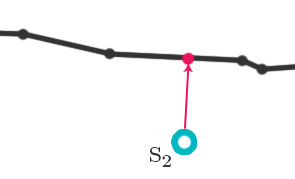
\includegraphics[width=0.25\textwidth]{find_nearest_point}
      \caption{Finde den am nächstgelegenen Punkt der Station auf der Polyline}
      \label{fig:find_nearest_point}
    \end{center}
  \end{figure}

  Nachdem ein Punkt auf der Polyline gefunden ist, kann die Distanz berechnet werden. Die Distanzen zweier Stationen $\{s_i,s_{i+1} \;|\; i \in \mathbb{N} \}$ sei $d_\triangle$. Diese kann jetzt wie folgt berechnet werden: $ d_\triangle = d_{i+1} - d_i$. 

  \begin{figure}[htbp]
    \begin{center}
      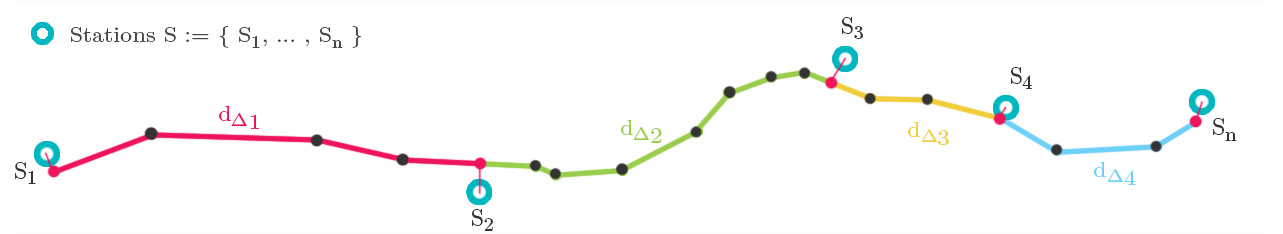
\includegraphics[width=\textwidth]{get_distances}
      \caption{Berechnen der Distanz}
      \label{fig:get_distances}
    \end{center}
  \end{figure}
  
  In Listing \ref{lst:match_station} des Anhangs wird ein Algorithmus vorgestellt, der das Problem des Station Matchings und der Distanzberechnung löst. Abbildung \ref{fig:station_matching_comparision} stellt eine frühere Implementierung mit der nun aktuellen Version des Algorithmus gegenüber. Dafür wird Zeit, die der jeweilige Algorithmus zum Matching über $n$-Trips benötigt verglichen. Um eine durchschnittliche Laufzeit zu erhalten wurde jeder Algorithmus 10 mal mit der gleichen Anzahl an Trips ausgeführt.

  \begin{figure}[htbp]
    \begin{center}
      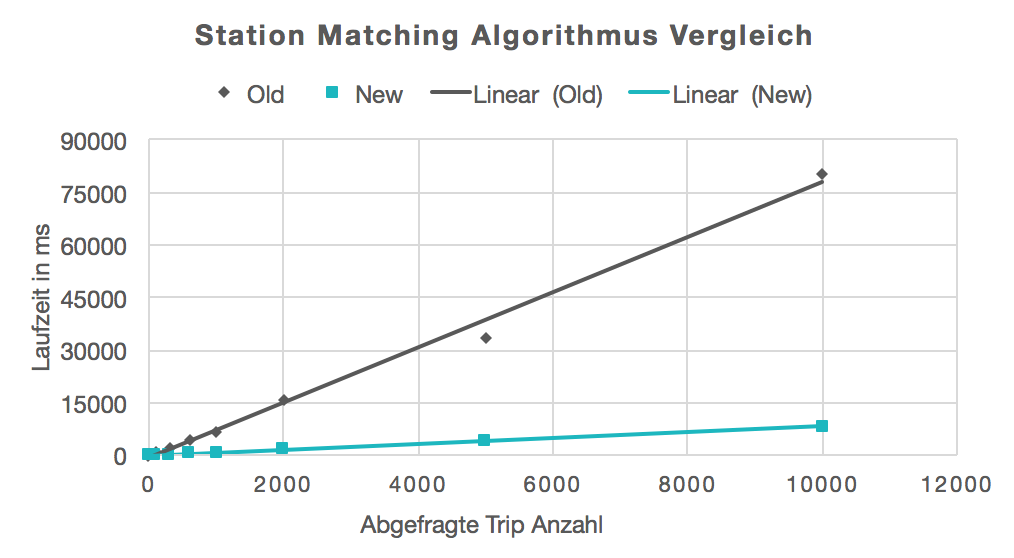
\includegraphics[width=0.7\textwidth]{station_matching_comparision}
      \caption{Vergleich der zwei Station Matching Algorithmen}
      \label{fig:station_matching_comparision}
    \end{center}
  \end{figure}

  Der alte Algorithmus war sehr simpel und beruhte darauf die Funktion \texttt{pointOnLine} der \texttt{Turf.js} Bibliothek zu verwenden. Diese Funktion hatte den entscheidenden Nachteil, dass sie in 3 \texttt{for}-Schleifen über die gesamten Punkte der Polyline iteriert. Hinzu kommt, dass das Matching nicht nur auf eine Station, sondern auf sämtliche Stationen aus allen Trips angewendet werden muss. Das führte dazu, dass insgesamt 5 \texttt{for}-Schleifen verwendet wurden. Damit lässt sich der im Vergleich höhere Anstieg der Laufzeit bei steigender Trip Anzahl erklären.

  Generell ist der neue Algorithmus sehr viel schneller. Durch die Verwendung eines \texttt{R-Trees}\footnotemark und der eigenen Implementierung verschiedener Bibliotheksfunktionen, konnte die Laufzeit drastisch reduziert werden (siehe Tabelle \ref{tbl:station_matching_comparison}). 

  \begin{longtable}{|>{\raggedright \arraybackslash}p{5.0cm}|>{\raggedright \arraybackslash}p{5.0cm}|>{\raggedright \arraybackslash}p{5.0cm}|}
  \caption{Station Matching Vergleich Old / New}\label{tbl:station_matching_comparison}\\
    \hline
    Anz. verarbeiteter Trips & Old (in ms)& New (in ms)\\
    \hline
    100    & 712   & 121  \\
    300    & 2191  & 305  \\
    600    & 4344  & 545  \\
    1.000  & 6780  & 874  \\
    2.000  & 15782 & 1700 \\
    5.000  & 33708 & 4161 \\
    10.000 & 80291 & 8279 \\
    \hline
  \end{longtable}

  Zwar wachsen beide Implementierungen lediglich Linear mit steigender Trip Anzahl, allerdings benötigt der neue Algorithmus für die Verarbeitung von $10.000$ Tausend Trips anstatt $80.29$ nur $8.28$ Sekunden.  

  Im Realbetrieb verarbeitet der Server zwischen $0 - 500$ Trips. Bei dieser Anzahl beträgt die Laufzeit des Algorithmus $\approx80ms - 400ms$. Dadurch kann argumentiert werden, dass der Algorithmus gerade noch schnell genug für eine Webanwendung arbeitet. Auch größere Anzahlen an Trips wären noch in akzeptabler Geschwindigkeit berechenbar. So können $1000$ Trips immer noch in unter einer Sekunde berechnet werden. Allerdings wäre es bei einer größeren Anzahl an Trips, der falsche Ansatz diese bei jeder Serveranfrage zu kalkulieren. Besser wäre es, einmalig das Matching für alle Trips eines GTFS Feeds durchzuführen und die Ergebnisse persistent in der Datenbank abzuspeichern. Dies könnte beispielsweise gleich beim Importieren der Daten in die Datenbank geschehen. Dadurch kann die Berechnung komplett eingespart werden. Da für das Stuttgart-VVS Feed glücklicherweise die zurückgelegte Distanz bis zu einer Station, bereits zur Verfügung steht, muss nur noch die Distanz zwischen den Stationen ($d\triangle$) berechnet werden. Dies geschieht nach dem selben Prinzip wie in der oben genannten Formel: $ d_\triangle = d_{i+1} - d_i$. Diese Berechnung ist trivial und erfolgt bei $10.000$ Trips in unter 15 Millisekunden.

  \footnotetext{Ein R-Tree (R für Rectangle) bezeichnet eine Baumförmige Datenstruktur für das Speichern und Abfragen von raumbezogenen Informationen. In Verwendung ist folgende Bibliothek: \url{https://github.com/mourner/rbush}}
  
% subsubsection station_matching (end)
  \subsubsection{Backend Performance}
\label{ssub:backend_performance}
  In diesem Abschnitt soll das gesamte Backend (Server und Datenbank) evaluiert werden. Dazu werden sowohl die Zeit zum Abfragen der Datenbank, als auch die Zeit zur Datenverarbeitung auf dem Server betrachtet werden.

  \begin{longtable}{|>{\raggedright \arraybackslash}p{4.5cm}|>{\raggedright \arraybackslash}p{1.2cm}|>{\raggedright \arraybackslash}p{1.2cm}|>{\raggedright \arraybackslash}p{1.2cm}|>{\raggedright \arraybackslash}p{1.2cm}|>{\raggedright \arraybackslash}p{1.2cm}|>{\raggedright \arraybackslash}p{1.2cm}|}
  \caption{Backend Evaluation}\label{tbl:backend_evaluation}\\
    \hline
    Anz. Trips & 20 & 100 & 500 & 1000 & 5000 & 10000\\
    \hline
    Query Zeit (ms)        & 25 & 88 & 124 & 200 & 855 & 1631 \\
    Verarbeitungszeit (ms) & 2 & 27 & 40 & 142 & 226 & 435 \\
    Summe (ms)             & 27 & 115 & 164 & 342 & 1081 & 2066 \\
    \hline
  \end{longtable}

  In Tabelle \ref{tbl:backend_evaluation} sind die Datenwerte für verschiedene Abfragen aufgelistet. Die Werte ergeben sich aus dem Mittelwert der Laufzeit in 10 Durchläufen. Wie bereits in Kapitel "`\nameref{ssub:bewältigung_der_datenmenge}"' festgestellt:

  \begin{quote}
    \textit{"`In einer Minute [werden] minimal 0 und maximal 27 Vehicle aktiv. Im Schnitt starten 9 Vehicles pro Minute ihre Fahrt."'}\ref{ssub:bewältigung_der_datenmenge}
  \end{quote}

  Aus dieser Aussage plus den gemessenen Werten lässt sich folgende Schlussfolgerung ziehen: Bei einer Anzahl zwischen 20 und 100 Trips reagiert der Server innerhalb von 25 bis $120ms$. Da die meisten Trips in diese Spanne fallen, ist dieses Ergebnis am bedeutendsten. 

  Im Bereich von 100 bis 500 Trips ist eine Antwortzeit von 115 bis $164ms$ immer noch sehr gut. Diese Anzahl an Trips ist dann relevant, wenn die Applikation das erste mal aufgerufen wird und die Karte noch leer ist. In diesem Fall kann es sein, dass der Server (je nach Datum und Uhrzeit) zwischen 200 - 500 Trips verarbeiten muss. Aber selbst Abfragen von bis zu 10.000 Trips, was ungefähr einer Zeitspanne von einem Tag gleich kommt, sind immer noch innerhalb von 2 Sekunden verarbeitet.\\

  Abschließend kann gesagt werden, dass in dieser Arbeit ein performantes Backendsystem für eine Web Applikation entwickelt worden ist, welches Serveranfragen effizient be- und verarbeiten kann.

  % \ref{sub:bewältigung_der_datenmenge}

% subsubsection backend_performance (end)
  % \subsubsection{Konfigurierung}
\label{ssub:konfigurierung}
  \begin{itemize}
    \item Why optimize
    \item What can be optimize
    \item A-B test of configuration
    \item Discuss test results
  \end{itemize}
% subsubsection konfigurierung (end)
% subsection backend (end)